\documentclass[12pt,fleqn]{article}\usepackage{../../common}
\begin{document}
Ders 14

Bağımsız Olmayan Değişkenler (Non-Independent Variables)

Örnek

Fizikteki $f(P,V,T)$ formülü, ki bu değişkenler 

$$ PV = nRT $$

şeklinde ilintili. Daha genel olarak bir $f(x,y,z)$ formülü var, ve
değişkenler $x,y,z$ birbiriyle $g(x,y,z) = c$ üzerinden bağlantılı. Aslında
bir önceki dersteki aynı durum, sadece bu sefer min, maks değil, kısmı
türevlere neler olduğunu inceleyeceğiz. 

Yine önceki dersteki gibi, belki $g$'yi cebirsel olarak değiştirip, $f$'e sokup
değişken yoketmek mümkün değil. Eğer öyle yapabilsek, bir $z = z(x,y)$
olabilirdi, ve onun kısmi türevlerine bakabilirdik,

$$ \frac{\partial z}{\partial x}, \frac{\partial z}{\partial y}, .. $$

gibi. Peki ya $z$'yi bulamıyorsak? Belki üstteki kısmi türevleri $z$'yi
bulmadan elde edebiliriz. 

Örnek

$$ x^2 + yz + z^3 = 8 $$

$(2,3,1)$ noktasına bakalım (yerine koyunca hakikaten 8 çıktığını
görüyoruz). Fakat bu değerlerde azıcık değişiklik yapınca, $z$ nasıl
değişir? Bu soruyu nasıl cevaplarım? 

Formülden $z$'yi çekip çıkarmak gerekir, küpsel (cubic) formüllerde bunu
yapmanın bir yolu var, fakat çok karmaşık bir formül ortaya
çıkartıyor. Aradığımız sonuca ulaşmanın daha kolay bir yolu var. 

$g$'nin tam diferansiyeline, yani $dg$'ye bakalım (üstteki formülü $g$
kabul ediyoruz). Tam diferansiyel

$$ 2x dx + z dy + (y+3z^2) dz = 0$$

Sağ taraf sıfır çünkü üstteki $g$ bir sabite eşit, $g=8$, sabitin değişimi
sıfır, yani $dg=0$. 

Tam diferansiyele $(2,3,1)$ değerini verelim

$$ 4dx + dy + 6dz = 0 $$

Bu formül bize her değişkenin değişiminin diğeri ile nasıl bağlantılı
olduğunu gösteriyor. Mesela $dx$ ve $dy$'yi biliyorsak, $dz$'yi, yani
$z$'nin değişimini hesaplayabiliriz. Yani $z=z(x,y)$ üzerinden 

$$ dz = -\frac{1}{6}(4dx + dy) $$

Bu formül bize kısmi türevleri de göstermiş oluyor aslında, çünkü tam
diferansiyel formülünde kısmi türevler vardır, üstteki formülde $dx,dy$'nin
yanında yer alan değerler onlardır. O zaman

$$ \frac{\partial z}{\partial x} = -\frac{4}{6} = -\frac{2}{3} $$

$$ \frac{\partial z}{\partial y} = -\frac{1}{6} $$

Bunu düşünmenin bir diğer yolu şu. $\partial z/\partial x$ $z$'nin $x$'e
göre değişimi ise, $y$ sabit demektir, üstteki $dz$ formülünde $dy=0$
deriz, geri kalanlar

$$ dz = -\frac{2}{3}dx $$

ki bu formül $z$'nin $x$'teki değişime göre nasıl değiştiğini gösteriyor. 

Genel olarak 

$$ g(x,y,z) = c $$

ise, o zaman 

$$ dg = g_x dx + g_y dy + g_z dz $$

formülü sıfıra eşitlenir, ve bir diferansiyel diğerinin formunda elde
edilebilir. 

$$ dz = -\frac{g_x}{g_z}dx -\frac{g_y}{g_z}dy $$

O zaman $\frac{\partial z}{\partial x}$'i görmek istiyorsak, 
$dx$'in katsayısına bakabiliriz, ya da $y=sabit$ yani $dy=0$ deriz, 
ve geri kalanlar

$$ dz =  -\frac{g_x}{g_z}dx, \ 
\frac{\partial z}{\partial x} = -\frac{g_x}{g_z}dx
$$

Daha fazla ilerlemeden, şimdiye kadar gördüğümüz notasyonun bazı
problemlerini inceleyelim. 

$$ f(x,y) = x+y $$

$$ \frac{\partial f}{\partial x} = 1$$

Değişken değişim (change of variables) yapalım

$$ x = u $$

$$ y = u+v $$

Pek çetrefil bir değişim değil bu. O zaman 

$$ f = x + y = 2u + v $$

$$ \frac{\partial f}{\partial u} = 2$$

Bu nasıl oldu? $x=u$ dediğimize göre, $x,u$ birbiriyle eşitler, o zaman
kısmi türevleri de aynı olmalıydı. 

Bu uyuşmazlığın niye ortaya çıktığını anlamak için notasyonun ne demek
istediğine yakından bakmamız lazım. $\partial f/\partial x$ ile $x$'i 
değiştiriyor, 
ama $y$'yi sabit tutuyoruz. $\partial f/\partial u$ ile $u$'yu değiştiriyor, ama 
$v$'yi 
sabit tutuyoruz.

Yani evet, $x$ ile $u$'yu değiştirmek aynı şey olabilir, ama $v$'yi sabit
tutmak ile $y$'yi sabit tutmak aynı şey değildir. Çünkü mesela $y$'yi sabit
tutarsam ve $u$'yu değiştirirsem, $v$ de değişmelidir (ki biz bunu
istemiyoruz) $y = u+v$ ifadesindeki toplamının sabit kalması için. Ya da $v$ 
sabit ise ve $u$'yu değiştiriyorsam, $y$ değişecektir. 

Yani hoş, güzel, kısmi türev notasyonumuz neyin değiştiğini açıkça
göstermesine rağmen, neyin sabit tutulduğunu göstermediği için yanılgılara
yol açabiliyor. Bunu aklımızda tutmamız lazım. Örnekteki kısmı türevler
birbiriyle aynı değil çünkü 

$\partial f/\partial x$, $u=x$'i değiştir, ve $y$'yi sabit tut

$\partial f/\partial u$, $u=x$'i değiştir, ve $v = y-x$'i sabit tut

anlamına geliyor. 

Daha açık bir notasyon şöyle olabilir

$$ 
\bigg( \frac{\partial f}{\partial x}  \bigg)_y = \textrm { y sabit}
$$

$$ 
\bigg( \frac{\partial f}{\partial u}  \bigg)_v = \textrm { v sabit}
$$

Örneğe dönersek

$$ 
\underbrace{
\bigg( \frac{\partial f}{\partial x}  \bigg)_y 
}_{1} 
\ne 
\underbrace{
\bigg( \frac{\partial f}{\partial x}  \bigg)_v = 
\bigg( \frac{\partial f}{\partial u}  \bigg)_v 
}_{2}
$$

Örnek
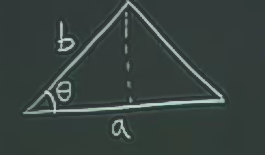
\includegraphics[height=3cm]{14_1.png}
$$ A = \frac{1}{2}ab \sin(\theta) $$

Alan, $a,b,\theta$'nin fonksiyonu. 

Farz edin ki size $a,b,\theta$ arasında bir ilişki olduğunu söyledim. 

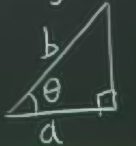
\includegraphics[height=3cm]{14_2.png}

Diyelim ki üçgen aslında bir dik üçgen, bunu cebirsel olarak söylemenin yolu da
alttaki kısıtlama ifadesi

$$ a = b \cos(\theta) $$

İncelemek istediğimiz alanın $\theta$'ya olan bağlantısı, yani, mesela
$A$'nin değişiminin $\theta$'nin değişimine oranı nedir? Bunu hesaplamanın
3 yöntemi olabilir

1) $a,b,\theta$'yi bağımsız kabul et, o zaman

$$ \frac{\partial A}{\partial \theta} = 
\bigg( \frac{\partial A}{\partial \theta} \bigg)_{a,b}  $$

Tabii $a,b$ sabitken $\theta$ değişsin demek, üçgenin dikliğinin ihlali
demektir, çünkü hem kenarlar sabit, hem açı değişsin diyoruz, ama o zaman
dik açı değişmek zorundadır. Her neyse, kısmi türevleri hesaplayalım. 

$$ \frac{\partial A}{\partial \theta} = \frac{1}{2}ab \cos\theta $$

Şimdiye kadar kısıtlama ifadelerimi kullanmadım. 

2) $a$'yi sabit tutalım, $b$ değişebilsin, ki böylece dik açı yerinde
kalabilsin. 

$$ b = b(a,\theta) = \frac{a}{\cos(\theta)} $$

$$ \bigg( \frac{\partial A}{\partial \theta} \bigg)_{a}  $$

3) $b$'yi sabit tutalım, $a = a(b,\theta)$ değişsin, ki böylece dik açı yerinde
kalabilsin. 

$$ \bigg( \frac{\partial A}{\partial \theta} \bigg)_{b}  $$

Bunlardan bir tanesini hesaplayalım, mesela $\bigg( \frac{\partial A}{\partial 
\theta} \bigg)_{a} $.

Hesabı yapmanın üç değişik yolunu göreceğiz. 

0. Metot: $b$'yi yanlız bırak (cebirsel), ve diğer formüle sok

$$ a = b \cos \theta => b = \frac{a}{\cos\theta} = a \sec\theta$$

$$ A = \frac{1}{2} \ ab \sin\theta $$

$$ = \frac{1}{2} \frac{a^2 \sin \theta}{\cos \theta} $$

$$ = \frac{1}{2} a^2 \tan \theta $$

O zaman 

$$ \bigg( \frac{\partial A}{\partial \theta} \bigg)_{a} = 
\frac{1}{2}a^2sec^2(\theta)
$$

Bu arada $sec$, $1/\cos$ demektir, eğer ve onun türevini $1+tan^2$ olarak
biliyorsanız, o da aynı kapıya çıkar. 

Hoca bu metotu tavsiye etmiyor (onun için metot sayısına biraz espri yaparak
'sıfır' vermiş) çünkü her zaman yanlız bırakma, başka formüle sokma mümkün
olmayabilir.

1'inci Metot: Diferansiyelleri Kullan

Yapılacaklar şunlar

- $a$'yi sabit tut, $da = 0$

- kısıtlama ifadesi $a = b \cos\theta$

Üstteki ifadenin diferansiyelini alalım

$$ da = \cos \theta db - b \sin\theta d\theta $$

Şimdi elimizde $da,db,d\theta$'yi ilişkilendiren bir ifade var. $a$'nin
sabit olduğunu biliyoruz, o zaman $da=0$

$$ 0 = \cos \theta db - b \sin \theta d\theta $$

$db$'yi yanlız bırakabiliriz

$$ \cos\theta db = b \sin\theta d\theta $$

$$ db = b \sin\theta d\theta \ / \cos\theta $$

$$ db = b \tan\theta d\theta  $$

Böylece $b$'nin $\theta$'ya göre değişim oranını bulduk. Bu ne ise yarar?
Ana formülü hatırlayalım, ve onun da diferansiyelini alalım

$$ A = \frac{1}{2} \ ab \sin\theta $$

$$ dA = \frac{1}{2} \ b \sin\theta da + 
\frac{1}{2} \ a \sin\theta db + 
\frac{1}{2} \ ab \cos\theta \ud \theta
 $$

$da = 0$ ise, ilk terim yokolur. 

$$ dA = 
\frac{1}{2} \ a \sin(\theta) db + 
\frac{1}{2} \ ab \cos \theta \ud \theta
$$

Geri kalanlarda, $db$ var, ama biz $\theta$'ya göre değişimi istiyoruz,
$db$'yi orada görmek istemiyoruz. O zaman elimizdeki $db$ formülünü buraya
sokalım. 

$$ dA =  
\frac{1}{2} \ a \sin\theta \ ( \ b \tan(\theta) d\theta \ ) \ + 
\frac{1}{2} \ ab \cos\theta \ud \theta
$$

$$ dA =  
\frac{1}{2} \ ab \ (\sin\theta \tan\theta +  \cos\theta )d\theta
$$

Trigonometriden 

$$ dA =  
\frac{1}{2} \ ab \ (
\underbrace{\sin(\theta) \tan(\theta) +  \cos \theta}_{sec(\theta)}
)d\theta
$$

Sonucu bulduk 

$$ \bigg( \frac{\partial A}{\partial \theta} \bigg)_{a} = 
\frac{1}{2} \ ab \ sec(\theta)
$$

Özetlemek gerekirse, şunları yaptık

- $A$'yi $da,db,d\theta$ ile ifade et

- $a=sabit, \ud a=0$ demektir.

- Kısıtlama ifadesinin diferansiyelini al, $db$'yi yanlız bırak. 

- $dA$'ya sok

2. Metot: Zincirleme Kanununu Kullan

$$ \bigg( \frac{\partial A}{\partial \theta} \bigg)_{a} = 
A_\theta \bigg( \frac{\partial \theta}{\partial \theta} \bigg)_{a} + 
A_a \bigg( \frac{\partial a}{\partial \theta} \bigg)_{a} + 
A_b \bigg( \frac{\partial b}{\partial \theta} \bigg)_{a} 
$$

$$  = 
A_\theta \cancelto{1}{\bigg( \frac{\partial \theta}{\partial \theta} \bigg)_{a}} 
+ 
A_a \cancelto{0}{\bigg( \frac{\partial a}{\partial \theta} \bigg)_{a}} + 
A_b \bigg( \frac{\partial b}{\partial \theta} \bigg)_{a}
$$

Sıfır olan kısmı türev öyle oldu çünkü $a$ sabit dedik. Son terimdeki
kısmı türev için kısıtlama ifadesini kullanacağız.

Soru 2J-1 a)

$$ w = x^2+y^2+z^2, \ z = x^2+y^2 $$

için 

$$ \bigg( \frac{\partial w}{\partial y}  \bigg)_z $$

hesabını yapın, ve direk yerine geçirme (direct subsitution) tekniğini
kullanın. 

Cevap 

Üstteki notasyon tüm sabit tutulan değişkenleri hangileriyse göstermek
zorunda, burada sadece $z$'nin sabit tutulduğu söyleniyor, değişen $y$. O
zaman bağımlı değişken $x$ olmalıdır. Bu değişkeni yokedelim,

$$ z = x^2+y^2 $$

$$ x^2 = z - y^2 $$

Yerine koyalım

$$  w = (z-y^2)+y^2+z^2 $$

$$ = z + z^2 $$

O zaman kısmi türev

$$ \bigg( \frac{\partial w}{\partial y}  \bigg)_z  = 0$$

olacaktır. 

Soru 2J-2 (b) (i)

Üstteki $w$ için, 

$$ \bigg( \frac{\partial w}{\partial z}  \bigg)_y $$

hesabını yap ve zincirleme kanunu kullan. 

Cevap 

$$  \bigg( \frac{\partial w}{\partial z}  \bigg)_y  =
2x \  \bigg( \frac{\partial w}{\partial z}  \bigg)_y  +  2z
$$

Diğer yandan 

$$ z = x^2 + y^2 $$

var, bunun üzerinde de aynı türevi alalım. Tekrar düzenleyip istediğimiz
değişkeni belli bir tarafa almaya gerek yok, çünkü yerine geçirme tekniği
kullanmıyoruz. İki tarafın kısmi türevini alınca

$$ 1 = 2x  \bigg( \frac{\partial w}{\partial z}  \bigg)_y  $$

$$ \frac{ 1}{2x}  = \bigg( \frac{\partial w}{\partial z}  \bigg)_y  $$

Ana formülün kısmı türevinde üstteki formülü yerine koyalım

$$
\bigg( \frac{\partial w}{\partial z}  \bigg)_y  =
2x  \frac{1}{2x}  + 2z
$$

$$   =
1 + 2z
$$

Soru 2J-4 b)

$$ w = x^3y - z^2t, \quad xy = zt$$

için

$$ \bigg( \frac{\partial w}{\partial t}  \bigg)_{x,z}  $$

hesabını yap, tam diferansiyel tekniğini kullan. 

Cevap

Çözüm için her iki denklemin tam diferansiyelini alacağız. Bağımlı,
bağımsız bilgisi ise ``diferansiyel yerine geçirme'' uyguladığımızda ise
yarayacak, yani daha önce düz değişken üzeinden yaptığımız değişimi, şimdi
diferansiyeller üzerinden yapacağız. Tam diferansiyeli mekanik bir şekilde
önce yazalım

$$ dw = w_x dx + w_y dy + w_z dz + w_t td $$

Gerekli kısmi türevleri alalım

$$ = 3x^2y dx + x^3dy - 2zt dz + -z^2 dt$$

Aynısı ikinci denklem için 

$$ y dx + x dy = t dz + z dt $$

Bizden istenene göre $t,x,z$'nin bağımsız, geri kalan $y$'nin bağımlı
olduğunu anlıyoruz. O zaman üstteki formülde $dy$'yi yanlız bırakırsak ve
ana tam diferansiyel içinde yerine koyarsak, istediğimiz sonuca
erişeceğiz. 

$$ y dx  = t dz + z dt = x dy$$

Yerine koyalım, ve gruplayalım

$$ = 3x^2ydx + x^2(tdz + zdt - ydx) - 2ztdz - z^2dt $$

$$ = (3x^2y  - x^2y)dx + (x^2t-2zt)dz + (x^2z-z^2)dt  $$

$$ = (2x^2y) dx + (x^2t-2zt) dz + (x^2z-z^2)dt  $$

Aradığımız kısmı türev $t$'ye göre, o zaman üstteki tam diferansiyel
açılımında $dt$'nin katsayısına bakacağız. Orada $x^2x-z^2$ yazıyor, demek
ki aradığımız sonuç bu. 

$$ \bigg( \frac{\partial w}{\partial t}  \bigg)_{x,z} = x^2x-z^2 $$

Soru 2K-3 a)

Laplace Denklemi iki boyutta şöyle

$$ \frac{\partial^2 w}{\partial x^2} + 
\frac{\partial^2 w}{\partial y^2}  = 0
$$

Diyelim ki şu formda olmak üzere

$$ w = ax^2 + bxy + cy^2 $$

tüm çözümleri istiyoruz. Bu çözümü bulduktan sonra çözümün $c_1f_1(x,y) +
c_2f_2(x,y)$ olarak temsil edilebilecegini gösterin, ki $c_1,c_2$ rasgele
birer sabit ve $f_1,f_2$ özel birer polinom. Yani çözüm $f_1,f_2$'nin
lineer bir kombinasyonu olabilmeli.

Çözüm 

$$ w_{xx} = \frac{\partial }{\partial x} (2ax + 4) = 2a $$

$$ w_{yy} = \frac{\partial }{\partial y} (2cy) = 2c $$

Eğer Laplace'a göre $w_{xx} + w_{yy} = 0$ olması gerekiyorsa,

$$ 2a + 2c = 0 $$

$$ a = -c $$

olmalı. Şimdi ana formülde $a$ yerine $-c$ koyalım. 

$$ ax^2 + bxy -ay^2 $$

$$ = a(x^2-y^2) + bxy $$

Üstteki formül iki polinomun lineer kombinasyonu formatına girdi bile. İki
rasgele sabiti $a,b$ olarak görebiliriz, ve iki polinom

$$ f_1 = x^2-y^2 $$

$$ f_2 = xy $$

Soru 2K-4

Tek boyutlu dalga denklemi 

$$ \frac{\partial ^2w}{\partial x^2} = \frac{ 1}{c^2} 
\frac{\partial ^2w}{\partial t^2} $$

için $w = f(x+ct) + g(x-ct)$ fonksiyonun bir çözüm olduğunu gösterin. 

Cevap 

Ders 11'de gösterildiği gibi $f(u)$ gibi bir fonksiyonun türevini alırken
Zincirleme Kanunu gerekiyor, bu kanunu her iki terim üzerinde ayrı ayrı
uyguluyoruz,

$$ \frac{\partial w}{\partial x}  = 
\frac{\partial f}{\partial u}
\frac{\partial u}{\partial x} + 
\frac{\partial g}{\partial u}
\frac{\partial u}{\partial x} 
$$

$f$, $u$ bağlamında tek değişkene bağlıymış gibi görülebilir, o zaman
$\partial$ yerine $d$ kullanılabilir, ya da $'$. 

$$ \frac{\partial w}{\partial x}  = 
\frac{df}{du}
\frac{\partial u}{\partial x} + 
\frac{dg}{du}
\frac{du}{\partial x} 
$$

İşlemi yapalım

$$ w_x = f' + g' $$

Üstte hiçbir $x,t$ ifadesi kalmadı, çünkü $x+ct$ ya da $x-ct$'nin $x$'e
göre göre türevi 1 sadece. Bir daha türev alırsak

$$ w_{xx} = f'' + g'' $$

$$ w_t = f'c - g'c $$

Üstteki türevde $u$ üzerinden tekrar Zincirleme Kanunu uygulandığına
dikkat. Çünkü $f'$ türev olmasına rağmen hala $u$'nun bir fonksiyonu hala.

$$ w_{tt} = f'c^2 + g'c^2 $$

Yerine koyarsak dalga denklemindeki eşitliğin doğru olduğunu görürüz. 

İlginç olan $f,g$'nin gösterilen $u$'ları içerdiği takdirde, herhangi bir
fonksiyon olabileceğidir. Daha fazla detay için PDE Ders 1 notlarına
bakılabilir.


\end{document}



